\chapter{अपनी दुनिया के अनुरूप}\label{ch:g4:adapted-to-their-world}

ध्रुवीय भालू को सहारा में रख दो और ऊँट को बर्फ़ की चादर पर, और दोनों
में से कोई एक मौसम भी न टिके। फिर भी अपने-अपने घर में हर एक उस्ताद है:
भालू बर्फ़ीले समुद्रों में आराम से तैरता है, और ऊँट वे रेगिस्तान पार कर
जाता है जो किसी घोड़े को दिनों में ख़त्म कर देते। \omterm{def:g1:living-or-not:living}{सजीव} अपनी दुनिया में
इतनी सटीकता से बैठते हैं कि ग़ौर से देखना पूरा मोल चुका देता है ---
ख़ासियत दर ख़ासियत।

\section{अनुकूलन का अर्थ}

\begin{definition}[अनुकूलन]\label{def:g4:adapted-to-their-world:adaptation}
\emph{अनुकूलन}\index{अनुकूलन} किसी \omterm{def:g1:living-or-not:living}{सजीव} के शरीर या व्यवहार की वह
ख़ासियत है जो उसे उसके \omterm{def:g2:caring-for-nature:environment}{पर्यावरण} की परिस्थितियों के अनुरूप बैठा देती है
--- ठंड या सूखे के, उसके भोजन के, उसके शिकारियों के अनुरूप।
\Cref{prop:g2:where-animals-live:fit} ने \omterm{def:g1:animals-around-us:animal}{जंतुओं} को अपने \omterm{def:g2:where-animals-live:habitat}{आवासों} में
बैठते दिखाया था; अनुकूलन वही बैठना है, टुकड़ा-टुकड़ा करके देखा हुआ।
\end{definition}

\begin{example}[ऊँट, टुकड़ा-टुकड़ा]\label{ex:g4:adapted-to-their-world:camel}
रेगिस्तान की समस्याएँ: गरमी, पानी नहीं, नरम रेत। ऊँट के उत्तर: चरबी के
कूबड़ --- सूखे सफ़रों के लिए \omterm{def:g3:animals-through-seasons:active}{भोजन-भंडार}; मिनटों में सौ लीटर पानी पी
लेने और फिर दिनों बिना पिए चलने की ताक़त; चौड़े, दो उँगलियों वाले पैर
जो रेत में धँसते नहीं; उड़ती धूल के सामने बंद हो जाने वाले नथुने, और
उनके साथ लंबी दोहरी पलकें। रेगिस्तान की हर समस्या के सामने एक ख़ासियत।
\end{example}

\begin{omfigure}
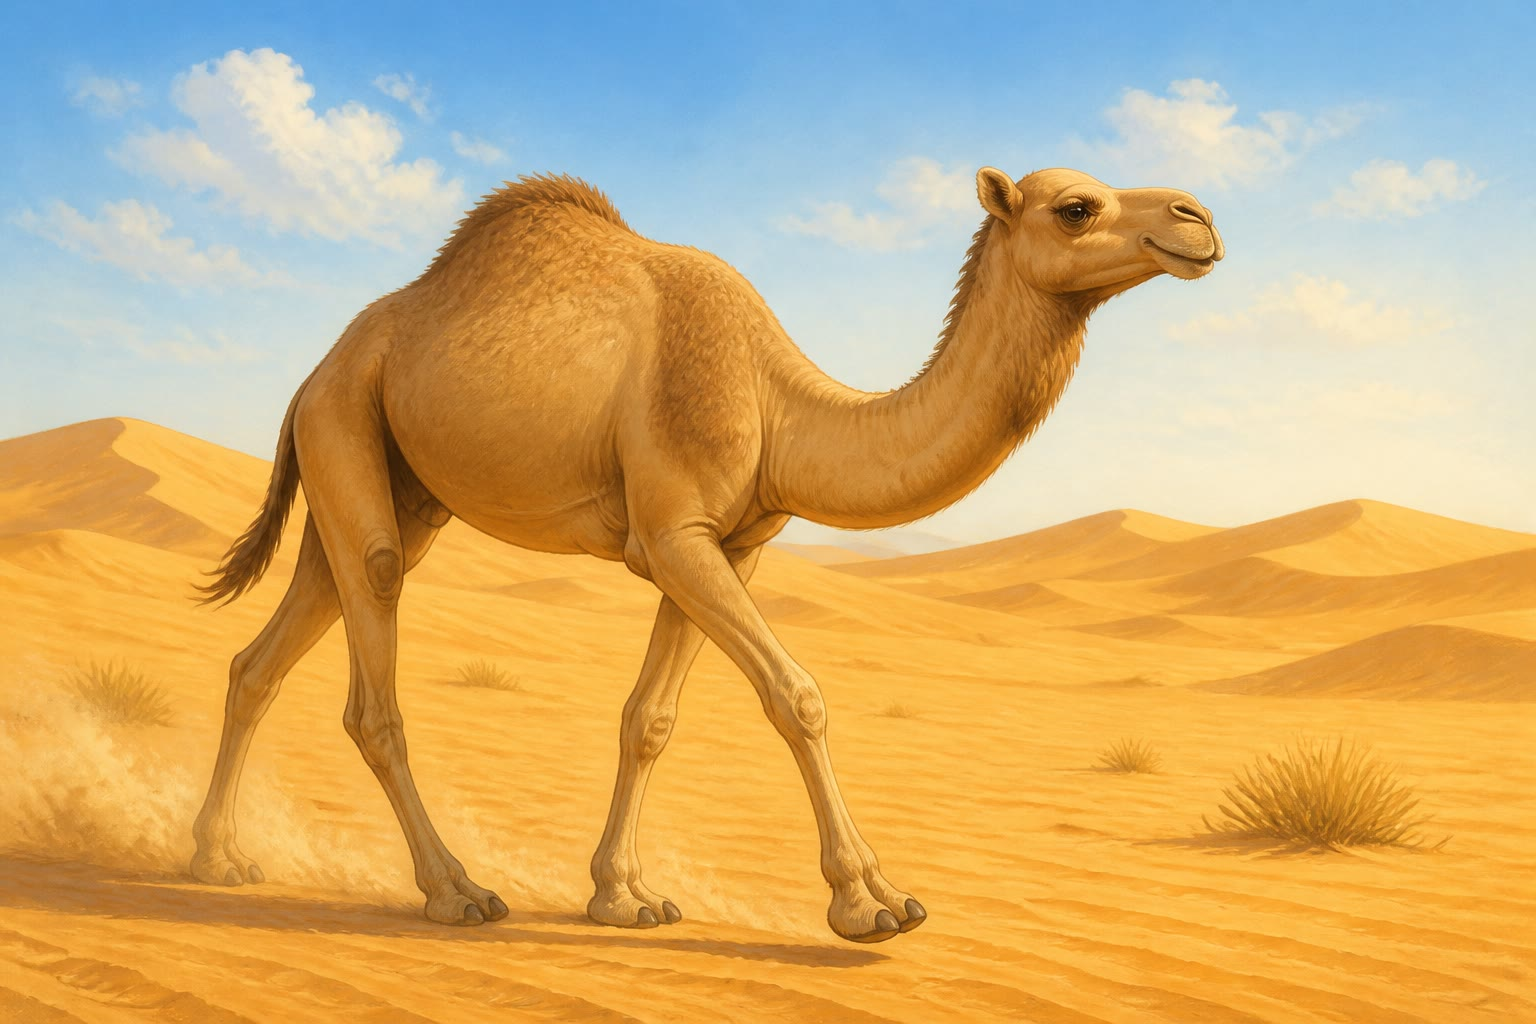
\includegraphics[width=0.6\linewidth]{images/book1/ai/g4-adapted-camel.jpg}

{\small रेगिस्तान का विशेषज्ञ काम पर: नरम रेत पर चौड़े पैर, भंडार का
एक कूबड़, और धूल के लिए बनी पलकें।}
\end{omfigure}

\begin{example}[ध्रुवीय भालू, टुकड़ा-टुकड़ा]\label{ex:g4:adapted-to-their-world:bear}
बर्फ़ की चादर की समस्याएँ: ठंड, बर्फ़ीला पानी, और सफ़ेद बर्फ़ पर ऐसा
शिकार जिसके पास पहुँचना मुश्किल है। भालू के उत्तर: चरबी की गहरी परत के
ऊपर मोटे \omterm{def:g1:animals-around-us:covering}{रोम} --- दोहरा कवच; चौड़े, हलके झिल्लीदार पंजे --- एक ही में
बर्फ़-जूते और चप्पू; सफ़ेद आवरण --- उसी बर्फ़ पर अदृश्य जिस पर वह शिकार
करता है। वही सटीकता, बस उलटी दुनिया के हिसाब से सधी हुई।
\end{example}

\begin{proposition}[अनुकूलन समस्याओं के उत्तर हैं]\label{prop:g4:adapted-to-their-world:answers}
जहाँ भी \omterm{def:g2:caring-for-nature:environment}{पर्यावरण} कोई कठिन समस्या रखता है, वहाँ बसे \omterm{def:g1:living-or-not:living}{सजीव} उसका उत्तर देने
वाली ख़ासियतें लिए रहते हैं:
\begin{itemize}
  \item ठंड: मोटे \omterm{def:g1:animals-around-us:covering}{रोम}, चरबी की परतें, छोटे \omterm{def:g1:the-five-senses:sense}{कान} जो कम गरमाहट गँवाते
        हैं;
  \item सूखा: पानी का भंडारण, मोम जैसी खालें, गहरी \omterm{def:g1:plants-around-us:parts}{जड़ें};
  \item पानी में जीवन: धारा-रेखित शरीर, मीन-पंख और झिल्लीदार पैर,
        पानी बहा देने वाले आवरण;
  \item चारों ओर शिकारी: छद्म रंग, कवच, काँटे, रफ़्तार, और चौड़ाई में
        लगी \omterm{def:g1:the-five-senses:sense}{आँखें} जो चारों ओर नज़र रखें;
  \item शिकार से रोज़ी: तेज़ इंद्रियाँ, आगे की ओर \omterm{def:g1:the-five-senses:sense}{आँखें}, पंजे और
        रफ़्तार (\cref{prop:g2:what-animals-eat:match})।
\end{itemize}
\end{proposition}
\admitted

\section{पौधे भी अनुकूलित हैं}

\begin{example}[नागफनी]\label{ex:g4:adapted-to-their-world:cactus}
रेगिस्तान \omterm{def:g1:plants-around-us:plant}{पौधों} की सबसे कड़ी परीक्षा लेता है --- वे चलकर पानी तक नहीं
जा सकते। नागफनी का उत्तर: एक मोटा, पीपे जैसा \omterm{def:g1:plants-around-us:parts}{डंठल} जो पानी जमा रखता है
और \omterm{def:g1:plants-around-us:parts}{पत्तियों} का प्रकाश पकड़ने का काम भी करता है; काँटों में सिमटी
\omterm{def:g1:plants-around-us:parts}{पत्तियाँ}, जो पानी लगभग बिलकुल नहीं गँवातीं --- और प्यासे \omterm{def:g1:animals-around-us:animal}{जंतुओं} से पीपे
की रक्षा भी करती हैं; और चौड़ी, उथली फैली \omterm{def:g1:plants-around-us:parts}{जड़ें}, जो दुर्लभ बौछार को एक
ही बार में पकड़ लें।
\end{example}

\begin{example}[पहाड़ी गद्दियाँ]\label{ex:g4:adapted-to-their-world:alpine}
ऊँचे पहाड़ों के \omterm{def:g1:plants-around-us:plant}{पौधे} जमा देने वाली हवा का सामना करते हैं। इनमें से कई
कसी हुई, ज़मीन से चिपकी गद्दियों के रूप में उगते हैं: गद्दी के भीतर हवा
टूट जाती है और वातावरण हलका नरम बना रहता है --- यानी आकार ही ओट है।
मैदानों में उगने वाले उन्हीं \omterm{def:g1:plants-around-us:plant}{पौधों} के सगे लंबे और खुले होते हैं;
पहाड़ी रूप चट्टान से चिपके रहते हैं।
\end{example}

\begin{method}[शरीर से जीव की दुनिया पढ़ना]\label{met:g4:adapted-to-their-world:read}
कोई अनजान \omterm{def:g1:animals-around-us:animal}{जंतु} या \omterm{def:g1:plants-around-us:plant}{पौधा} सामने हो, तो:
\begin{enumerate}
  \item उसकी उभरी हुई ख़ासियतें गिनाओ --- आवरण, पैर, \omterm{def:g1:the-five-senses:sense}{आँखें}, शरीर का
        आकार, \omterm{def:g1:plants-around-us:parts}{पत्तियाँ}, \omterm{def:g1:plants-around-us:parts}{जड़ें};
  \item हर एक के लिए पूछो: \emph{यह किस समस्या को हल करेगी?}
  \item उत्तरों को जोड़कर उसके घर की तस्वीर बनाओ --- ठंडा या गरम, नम
        या सूखा, शिकारी या शिकार;
  \item अपने अंदाज़े को इससे जाँचो कि वह जीव सचमुच रहता कहाँ है।
\end{enumerate}
यह \cref{met:g2:where-animals-live:matching} का बड़ा हो चुका रूप है:
\omterm{def:g2:where-animals-live:habitat}{आवास} मिलाने से आगे बढ़कर एक पूरी दुनिया फिर से खड़ी करना।
\end{method}

\begin{example}[किसी पहेली वाली खाल पर विधि]\label{ex:g4:adapted-to-their-world:mystery}
संग्रहालय की दराज़ में बिना नाम की एक खाल पड़ी है: घने मुलायम \omterm{def:g1:animals-around-us:covering}{रोम},
नन्ही \omterm{def:g1:the-five-senses:sense}{आँखें}, फावड़े जैसे विशाल अगले पंजे। \omterm{def:g1:animals-around-us:covering}{रोम} कहते हैं \omterm{prop:g3:sorting-living-things:groups}{स्तनधारी};
फावड़े कहते हैं खोदना; और बेकार-सी \omterm{def:g1:the-five-senses:sense}{आँखें} कहती हैं अँधेरे में जीवन।
फ़ैसला: ज़मीन के नीचे खोदने वाला जीव --- और सचमुच वह छछूँदर है
(\cref{ex:g2:where-animals-live:mole}), सिर्फ़ तीन ख़ासियतों से ठीक-ठीक
पढ़ा हुआ।
\end{example}

\begin{remark}[यह मेल बनता कैसे है?]\label{rem:g4:adapted-to-their-world:how}
ऊँट कभी \emph{तय} नहीं करता कि उसके चौड़े पैर उगें, और कोई ध्रुवीय
भालू अपना सफ़ेद आवरण नहीं चुनता। फिर \omterm{def:g1:living-or-not:living}{सजीव} अपनी दुनिया में इतनी अच्छी
तरह बैठते कैसे हैं? यह \omterm{def:g1:living-or-not:living}{जीवविज्ञान} के सबसे गहरे सवालों में से एक है, और
इसका पूरा उत्तर --- कि यह मेल पीढ़ी दर पीढ़ी कैसे बनता जाता है --- यह
पुस्तक आगे के किसी साल के लिए बचाकर रखती है। फ़िलहाल इस मेल को
\emph{देखना} सीखो: यह देखना ही वह चीज़ है जिसने उस सवाल को पूछने लायक़
बनाया।
\end{remark}

\section{अभ्यास}

\begin{exercise}[$\star$]\label{exo:g4:adapted-to-their-world:1}
\omterm{def:g4:adapted-to-their-world:adaptation}{अनुकूलन} क्या है? एक \omterm{def:g1:animals-around-us:animal}{जंतु} का और एक \omterm{def:g1:plants-around-us:plant}{पौधे} का उदाहरण दो।
\end{exercise}

\begin{exercise}[$\star$]\label{exo:g4:adapted-to-their-world:2}
रेगिस्तान की तीन समस्याएँ और हर एक पर ऊँट का उत्तर बताओ।
\end{exercise}

\begin{exercise}[$\star$]\label{exo:g4:adapted-to-their-world:3}
बर्फ़ की चादर की तीन समस्याएँ और हर एक पर ध्रुवीय भालू का उत्तर बताओ।
\end{exercise}

\begin{exercise}[$\star$]\label{exo:g4:adapted-to-their-world:4}
नागफनी के काँटे कौन-कौन से काम करते हैं? उसका पीपे जैसा \omterm{def:g1:plants-around-us:parts}{डंठल} क्या जमा
रखता है, और उसने कौन-सा काम अपने ऊपर ले लिया है?
\end{exercise}

\begin{exercise}[$\star$]\label{exo:g4:adapted-to-their-world:5}
ऊँचे पहाड़ों के बहुत-से \omterm{def:g1:plants-around-us:plant}{पौधे} कसी हुई गद्दियों के रूप में क्यों उगते हैं?
\end{exercise}

\begin{exercise}[$\star$]\label{exo:g4:adapted-to-their-world:6}
\cref{prop:g4:adapted-to-their-world:answers} से शिकार होने वाले
\omterm{def:g1:animals-around-us:animal}{जंतुओं} के दो और शिकारियों के दो \omterm{def:g4:adapted-to-their-world:adaptation}{अनुकूलन} बताओ।
\end{exercise}

\begin{exercise}[$\star$]\label{exo:g4:adapted-to-their-world:7}
\cref{ex:g4:adapted-to-their-world:mystery} दोहराओ: किन तीन ख़ासियतों
ने छछूँदर का भेद खोला, और हर एक ने क्या कहा?
\end{exercise}

\begin{exercise}[$\star$]\label{exo:g4:adapted-to-their-world:8}
करके देखो: कोई भी ऐसा \omterm{def:g1:animals-around-us:animal}{जंतु} चुनो जिसे तुम देख सको --- बत्तख़, बिल्ली,
मकड़ी --- और उस पर \cref{met:g4:adapted-to-their-world:read} चलाओ: तीन
ख़ासियतें, तीन हल की गई समस्याएँ।
\end{exercise}

\begin{exercise}[$\star\star$]\label{exo:g4:adapted-to-their-world:9}
रेगिस्तानी लोमड़ी के \omterm{def:g1:the-five-senses:sense}{कान} बहुत बड़े होते हैं; ध्रुवीय लोमड़ी के बहुत
छोटे। \cref{prop:g4:adapted-to-their-world:answers} की ठंड वाली पंक्ति
से दोनों समझाओ --- बड़े \omterm{def:g1:the-five-senses:sense}{कान} गरमाहट का क्या करते होंगे?
\end{exercise}

\begin{exercise}[$\star\star$]\label{exo:g4:adapted-to-their-world:10}
पहेली वाला एक \omterm{def:g1:animals-around-us:animal}{जंतु}: धारा-रेखित शरीर, झिल्लीदार पिछले पैर, घने पानी बहा
देने वाले \omterm{def:g1:animals-around-us:covering}{रोम}, मूँछें, और वह साँस अच्छी तरह रोक लेता है।
\cref{met:g4:adapted-to-their-world:read} से उसकी दुनिया फिर से खड़ी
करो। (वह बाँध बनाता है।)
\end{exercise}

\begin{exercise}[$\star\star\star$]\label{exo:g4:adapted-to-their-world:11}
ह्वेल (\cref{ex:g3:sorting-living-things:surprises}) मछली के आकार वाला
\omterm{prop:g3:sorting-living-things:groups}{स्तनधारी} है: धारा-रेखित, मीन-पंखों वाला, चिकना। ट्राउट उसी आकार की
मछली है। दो \emph{असंबंधित} तैराकों की यह समानता \omterm{def:g4:adapted-to-their-world:adaptation}{अनुकूलनों} के बारे में
क्या दिखाती है --- आकार किसने तय किया, कुल ने या पानी ने?
\end{exercise}
